\section{Results}

\begin{enumerate}
	\item plot lift and drag coeff histories for proof of convergence history for ALL Runs (appendix)
	\item Table of $C_l$, $C_d$, L/D, $C_m$
	\item plots of the items in the table and compared against Xfoil data at the closest Re \# (take directly from airfoiltools.com)
	\item streamlines and pressure contours to depict flow near airfoil
	\begin{itemize}
		\item 1 plot for each case
		\item use the same contour levels
	\end{itemize}
	\item y+ curves (for $0^\circ$ AoA case)
	\item plot showing turbulent boundary layer development ($0^\circ$ AoA case)
\end{enumerate}

\subsection{Plots of convergence history for all runs}
See Appendix A

\subsection{Table of final force/moment coefficient values}

\begin{table}[H]
\caption{Some aerodynamic coefficients}
\centering
\begin{tabular}{|l|l|l|l|l|} \hline
\textbf{AoA ($^\circ$)} & $\boldsymbol{C_l}$ & $\boldsymbol{C_d}$ & $\boldsymbol{C_m}$ & \textbf{L/D} \\ \hline \hline
-7           & -0.2475        & 0.0129         & -0.0317        & -19.1200     \\ \hline
-4           & 0.0771         & 0.0106         & -0.1102        & 7.3024       \\ \hline
-2           & 0.1864         & 0.0105         & -0.1368        & 17.7983      \\ \hline
0            & 0.5159         & 0.0106         & -0.0891        & 48.5390      \\ \hline
5            & 1.0736         & 0.0119         & -0.3562        & 90.3674      \\ \hline
8.5          & 1.4360         & 0.0173         & -0.4419        & 82.7872      \\ \hline
12           & 1.7358         & 0.0261         & -0.5071        & 66.4839      \\ \hline
14.5         & 1.8475         & 0.0381         & -0.5246        & 48.5187      \\ \hline
17           & 1.6456         & 0.0890         & -0.4857        & 18.4886      \\ \hline
19.5         & 1.3897         & 0.1635         & -0.4471        & 8.4988       \\ \hline
22           & 1.2712         & 0.2341         & -0.4433        & 5.4310       \\ \hline
\end{tabular}
\end{table}

\begin{figure}[H]
	\centering
	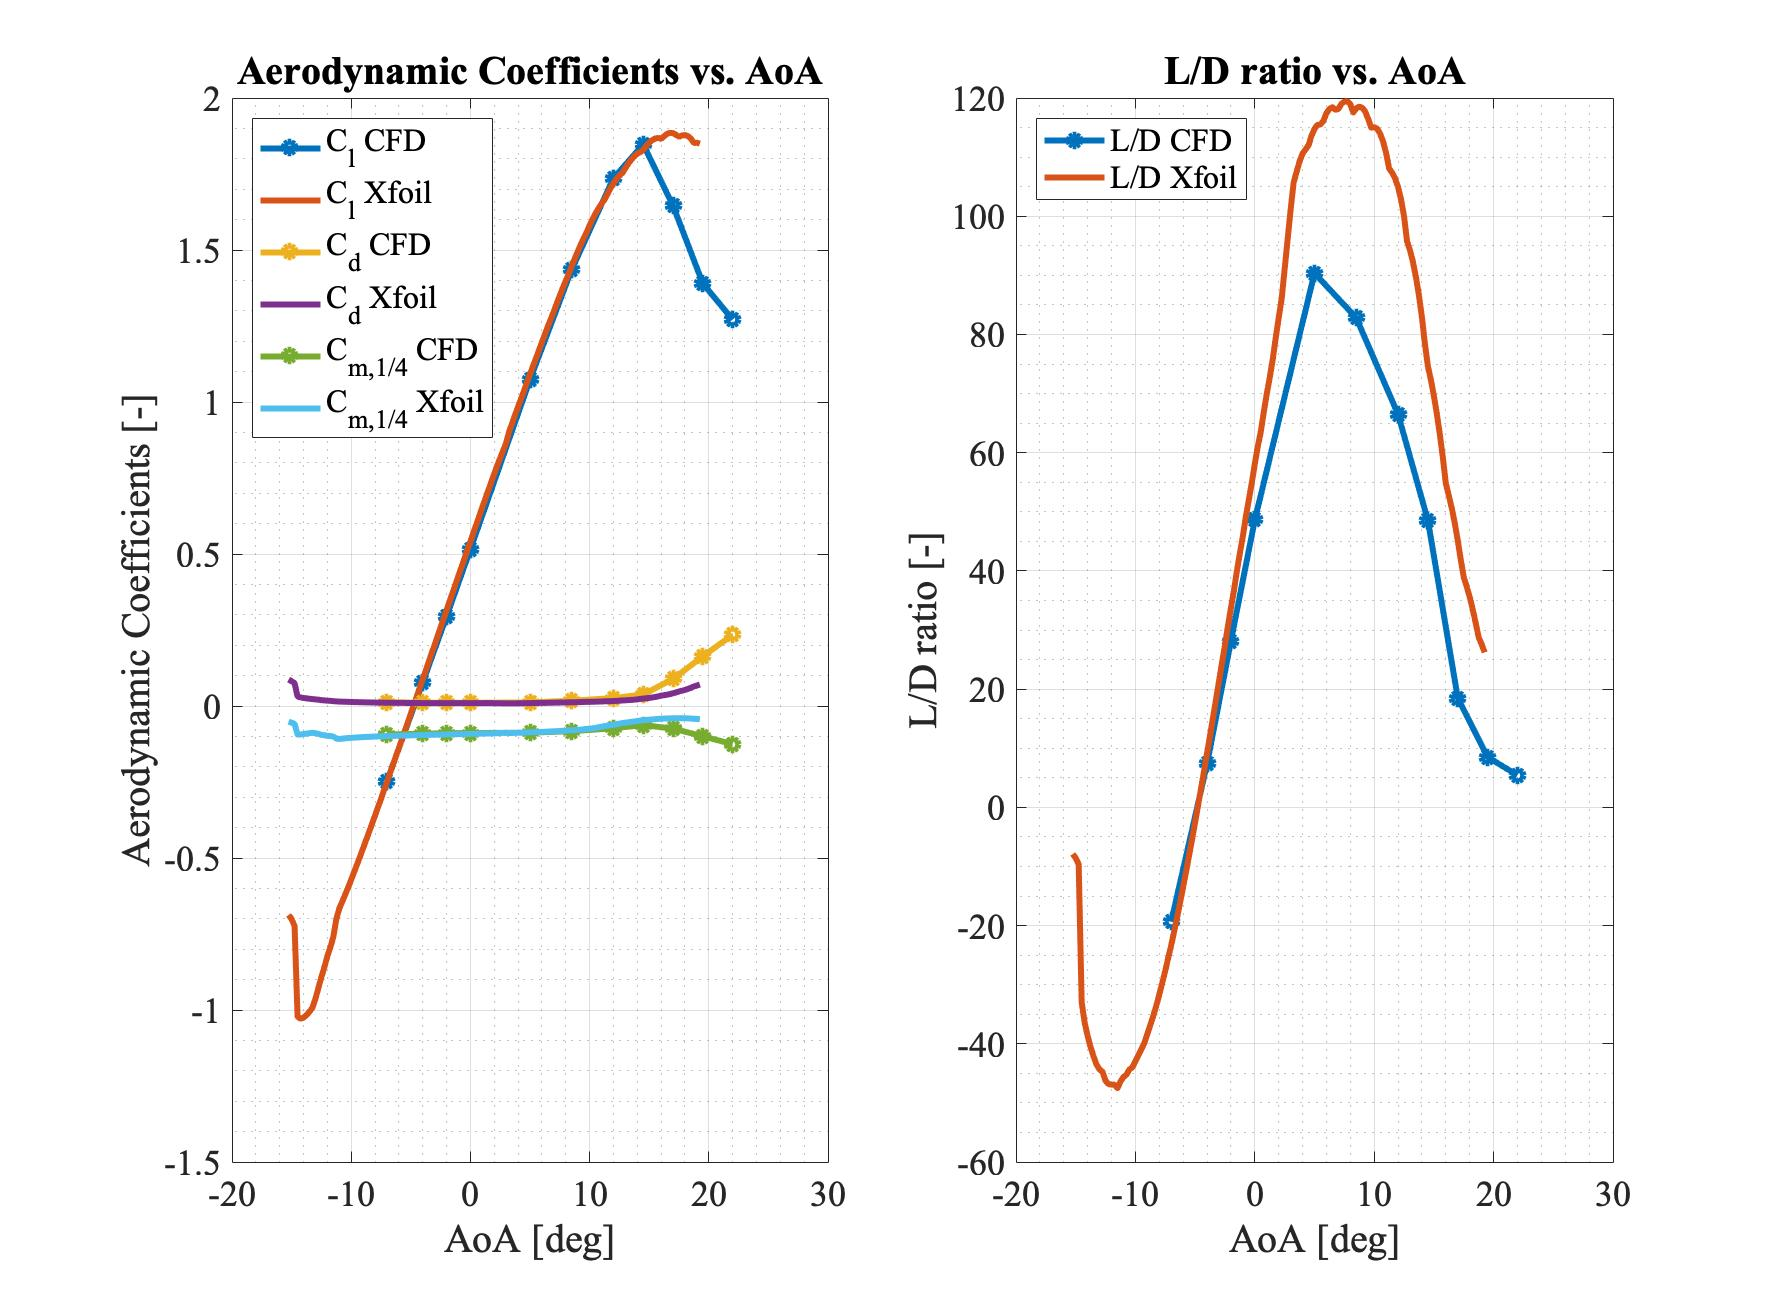
\includegraphics[width=\textwidth]{coeffs.jpg}
	\caption{Comparison of aerodynamic coefficients from Xfoil and CFD}
\label{fig:coeffs}
\end{figure}

\subsection{Pressure contours and streamlines}

\begin{figure}[H]
	\centering
	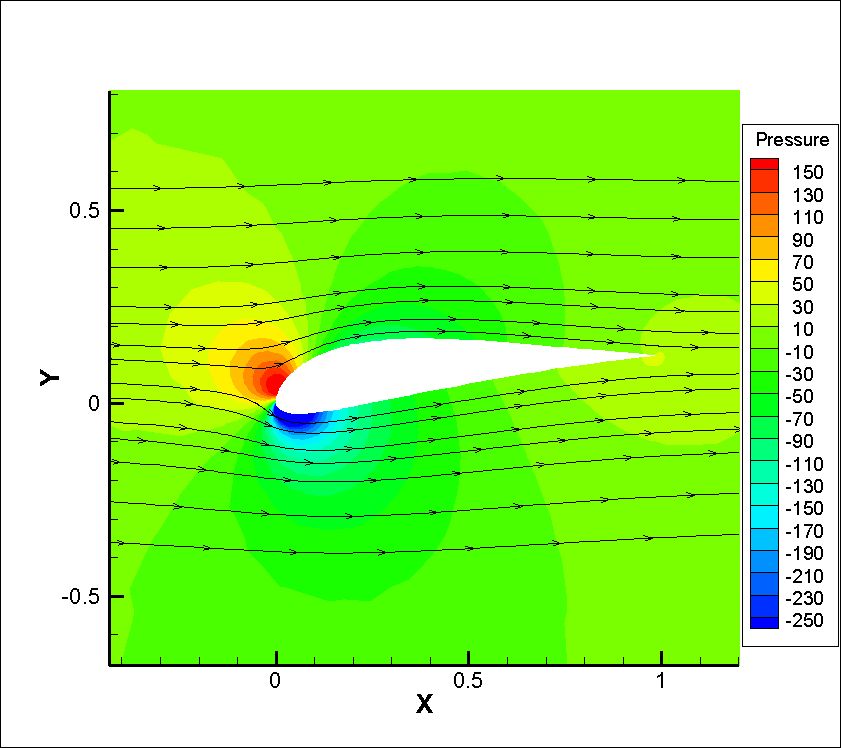
\includegraphics[width=0.6\textwidth]{tecplot_stuff/cont_stream_-7.png}
	\caption{Pressure contours and streamlines for AoA = -7$^\circ$}
\label{fig:cont_stream_-7}
\end{figure}

\begin{figure}[H]
	\centering
	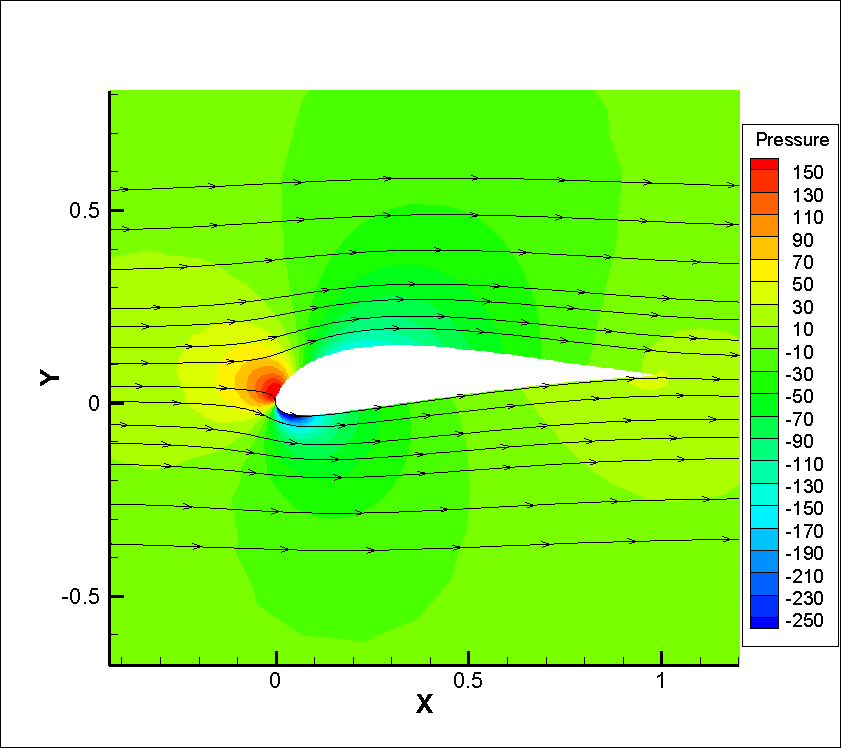
\includegraphics[width=0.6\textwidth]{tecplot_stuff/cont_stream_-4.png}
	\caption{Pressure contours and streamlines for AoA = -4$^\circ$}
\label{fig:cont_stream_-4}
\end{figure}


\begin{figure}[H]
	\centering
	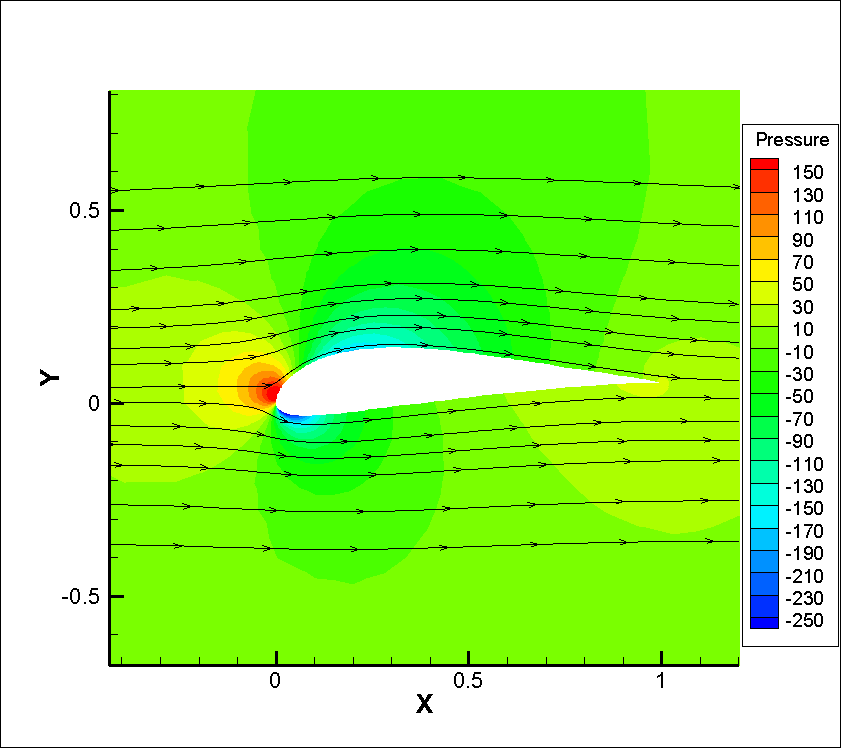
\includegraphics[width=0.6\textwidth]{tecplot_stuff/cont_stream_-2.png}
	\caption{Pressure contours and streamlines for AoA = -2$^\circ$}
\label{fig:cont_stream_-2}
\end{figure}


\begin{figure}[H]
	\centering
	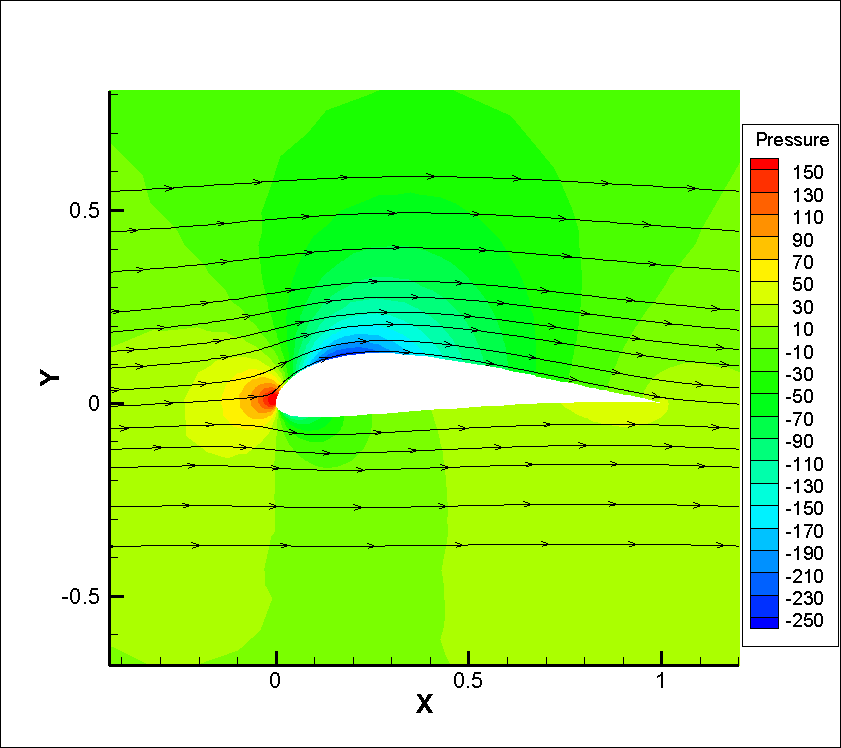
\includegraphics[width=0.6\textwidth]{tecplot_stuff/cont_stream_0.png}
	\caption{Pressure contours and streamlines for AoA = 0$^\circ$}
\label{fig:cont_stream_0}
\end{figure}


\begin{figure}[H]
	\centering
	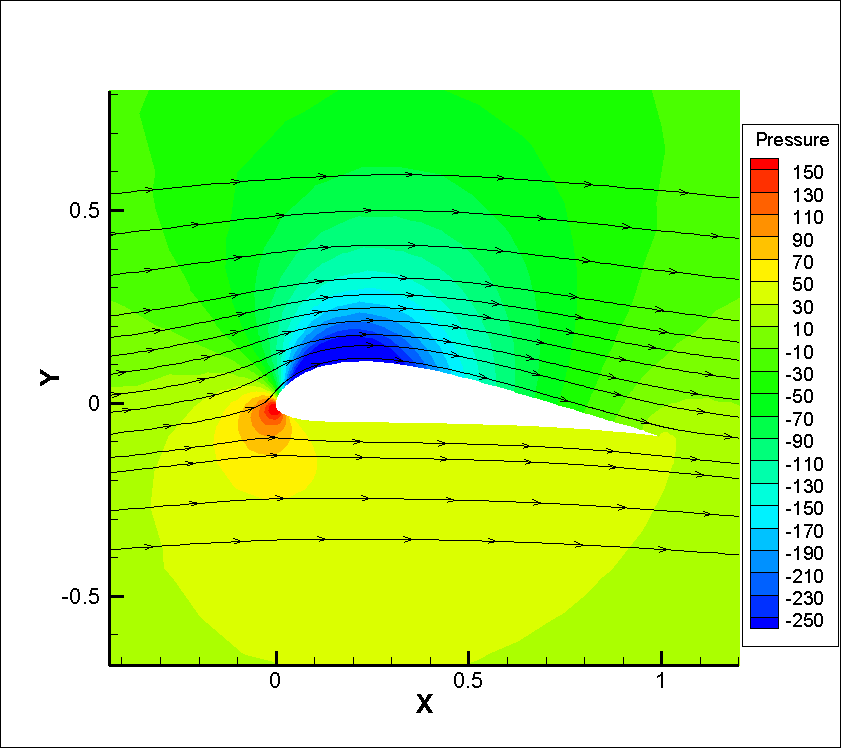
\includegraphics[width=0.6\textwidth]{tecplot_stuff/cont_stream_5.png}
	\caption{Pressure contours and streamlines for AoA = 5$^\circ$}
\label{fig:cont_stream_5}
\end{figure}


\begin{figure}[H]
	\centering
	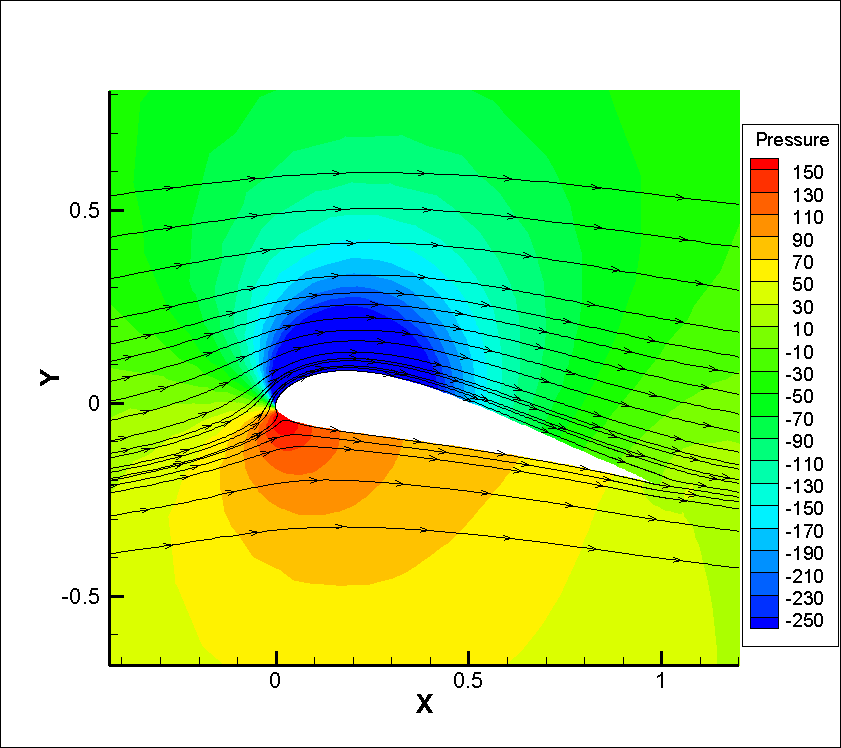
\includegraphics[width=0.6\textwidth]{tecplot_stuff/cont_stream_12.png}
	\caption{Pressure contours and streamlines for AoA = 12$^\circ$}
\label{fig:cont_stream_12}
\end{figure}

\begin{figure}[H]
	\centering
	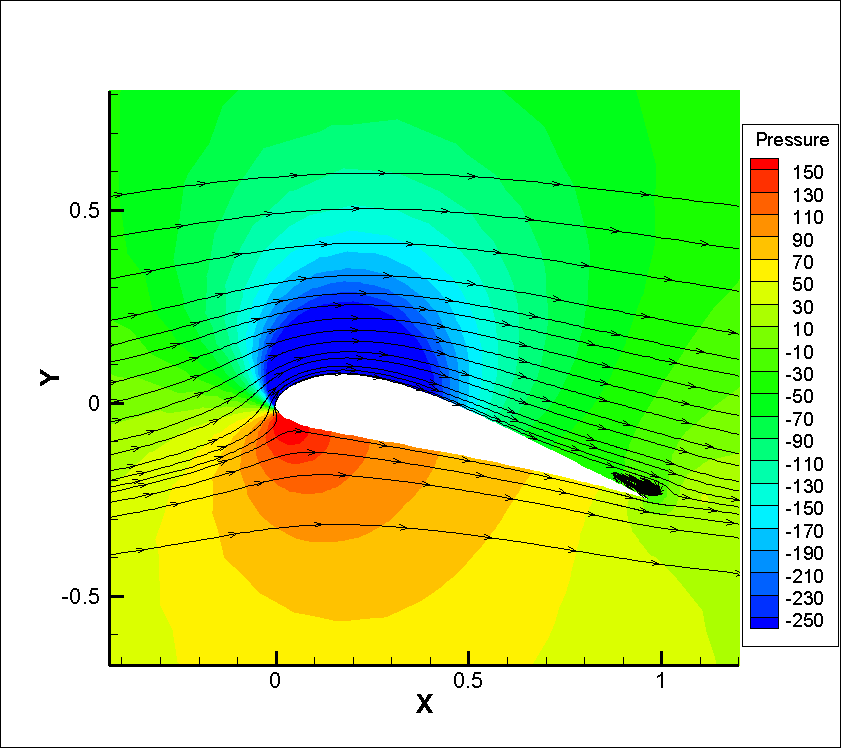
\includegraphics[width=0.6\textwidth]{tecplot_stuff/cont_stream_14_5.png}
	\caption{Pressure contours and streamlines for AoA = 14.5$^\circ$}
\label{fig:cont_stream_14_5}
\end{figure}

\begin{figure}[H]
	\centering
	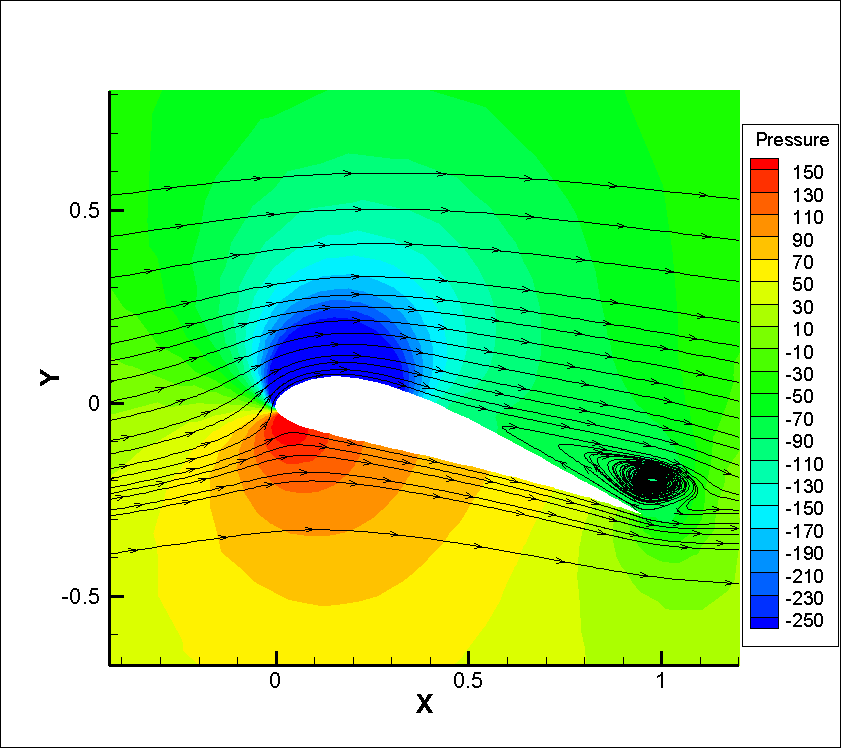
\includegraphics[width=0.6\textwidth]{tecplot_stuff/cont_stream_17.png}
	\caption{Pressure contours and streamlines for AoA = 17$^\circ$}
\label{fig:cont_stream_17}
\end{figure}

\begin{figure}[H]
	\centering
	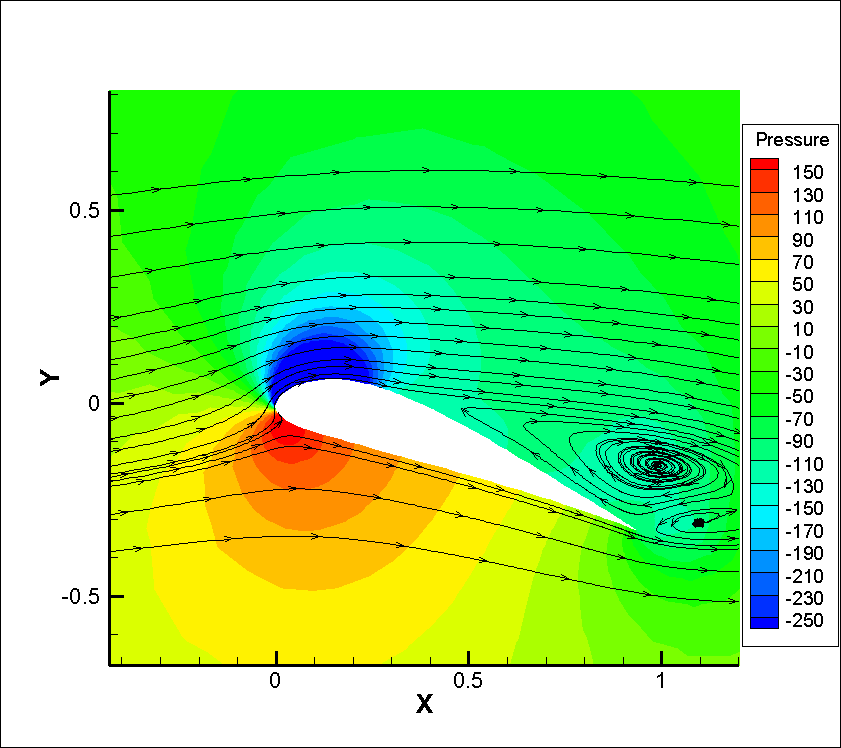
\includegraphics[width=0.6\textwidth]{tecplot_stuff/cont_stream_19_5.png}
	\caption{Pressure contours and streamlines for AoA = 19.5$^\circ$}
\label{fig:cont_stream_19_5}
\end{figure}

\begin{figure}[H]
	\centering
	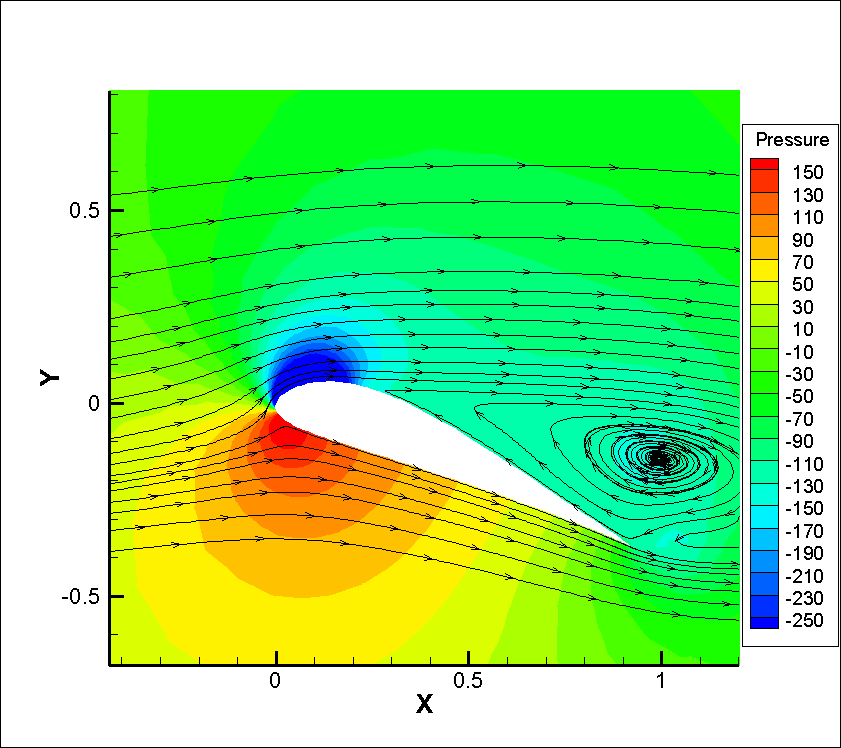
\includegraphics[width=0.6\textwidth]{tecplot_stuff/cont_stream_22.png}
	\caption{Pressure contours and streamlines for AoA = 22$^\circ$}
\label{fig:cont_stream_22}
\end{figure}

\subsection{y+ Curve}

\begin{figure}[H]
	\centering
	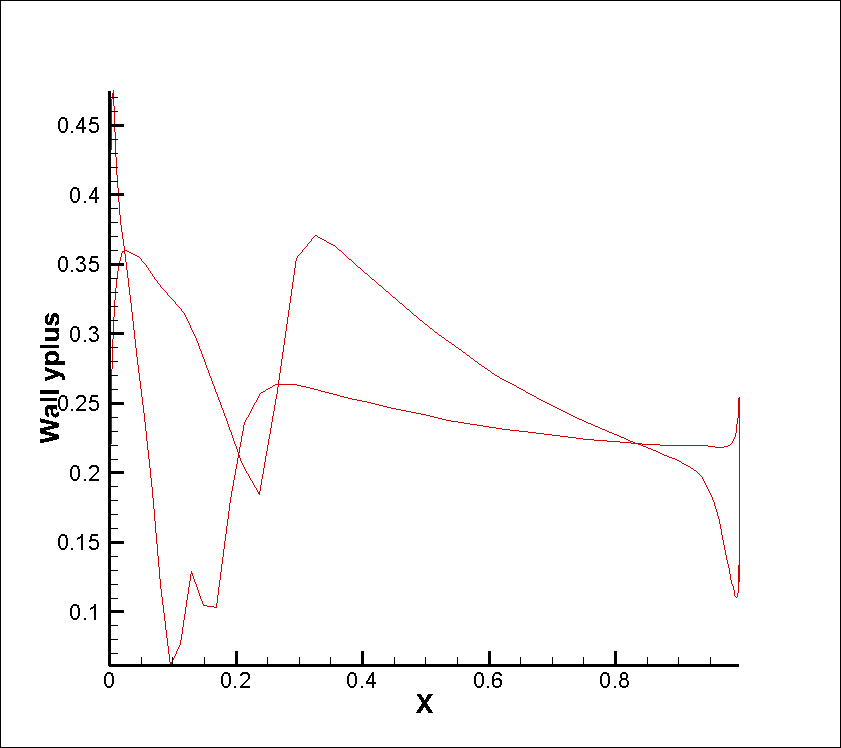
\includegraphics[width=0.6\textwidth]{tecplot_stuff/y_plus_0.png}
	\caption{y plus graph}
\label{fig:yplus}
\end{figure}

\subsection{Turbulent Boundary Layer Development}

\begin{figure}[H]
	\centering
	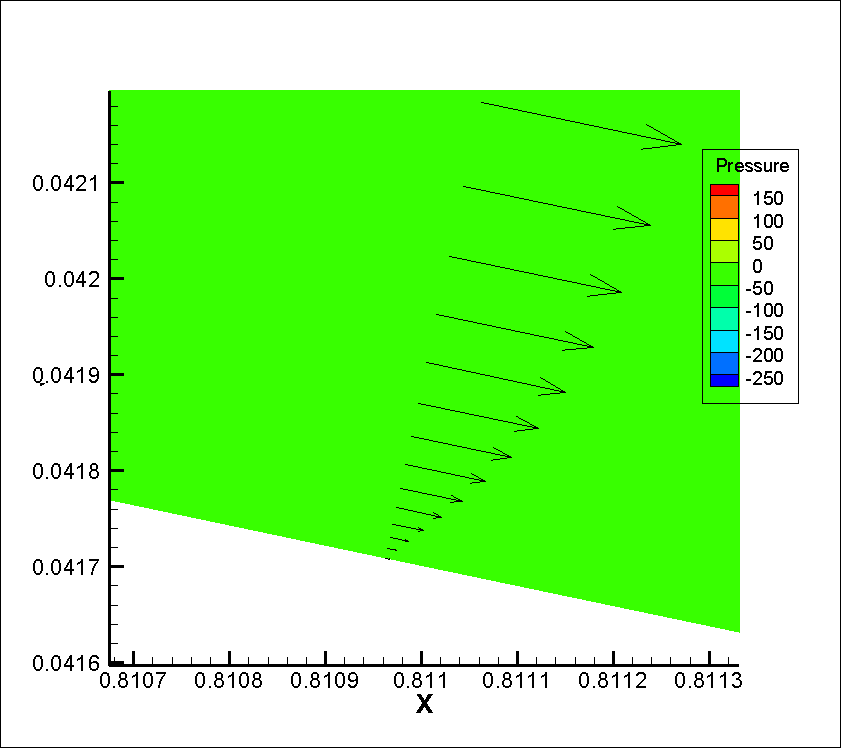
\includegraphics[width=0.6\textwidth]{tecplot_stuff/BL_0.png}
	\caption{Boundary layer near trailing edge of wing}
\label{fig:BL}
\end{figure}
